% ==============================================================================
% Monografia - Áurea Santos de Oliveira
% Capítulo 6 - A PoC como ferramenta de análise qualitativa
% ==============================================================================
\chapter{A Prova de Conceito como Ferramenta de Análise Qualitativa}
\label{sec-analise}

Um sistema de RAG costuma ser avaliado pelas respostas que produz. A resposta, porém, é o último elo de uma cadeia: antes dela, cada modalidade de busca decide o que recuperar, como organizar o que recuperou e o que efetivamente enviar ao modelo. Duas respostas parecidas podem ter origens muito diferentes, e uma resposta incompleta pode decorrer tanto de uma recuperação ruim quanto de um modelo que não aproveitou um bom contexto. Este capítulo mostra como a aplicação desenvolvida permite examinar essa cadeia. A Seção~\ref{sec-analise-grafo} analisa o próprio grafo de conhecimento gerado, que é a matéria-prima das modalidades baseadas em grafo. As seções seguintes examinam, modalidade por modalidade, consultas reais registradas no histórico.

As consultas analisadas são exemplos ilustrativos, escolhidos para exercitar cada modalidade com um tipo de pergunta adequado a ela, e não constituem uma avaliação comparativa: cada uma foi executada uma única vez, com perguntas diferentes, e o objetivo é mostrar o que a ferramenta torna visível. A avaliação sistemática entre modalidades é discutida como trabalho futuro no Capítulo~\ref{sec-conclusoes}.

%%% Início de seção. %%%
\section{O Grafo Resultante}
\label{sec-analise-grafo}

Antes de examinar o que cada consulta recupera, vale examinar o que há para ser recuperado. A exploração do grafo na aplicação -- com filtros por tipo, coloração por comunidade e o painel de detalhes das entidades -- e uma análise das tabelas do índice revelam características do grafo que ajudam a entender tanto o CDC quanto o comportamento das buscas.

\subsection{Poucas entidades centrais}
\label{sec-analise-grafo-centrais}

A distribuição dos graus é muito concentrada (Figura~\ref{fig-grafo-graus}). Metade das entidades tem até seis relações (média de 9,9), mas quatro entidades se destacam: CONSUMIDOR (597 relações), FORNECEDOR (272), PRODUTO (262) e SERVIÇO (218). São exatamente os quatro conceitos que o art. 2º e o art. 3º do CDC definem e sobre os quais todo o código se apoia. A entidade CONSUMIDOR foi extraída de 94 dos 130 artigos. Em seguida aparecem direitos transversais (DIREITO À INFORMAÇÃO, DIREITO À REPARAÇÃO DE DANOS), a tutela judicial (DEFESA DO CONSUMIDOR EM JUÍZO) e três artigos que são, eles próprios, listas: o art. 39, que enumera as práticas abusivas, o art. 6º, os direitos básicos, e o art. 51, as cláusulas abusivas. Artigos desse tipo se tornam centrais porque cada item da lista dá origem a uma entidade ligada ao artigo.

\begin{figure}[htb]
\centering
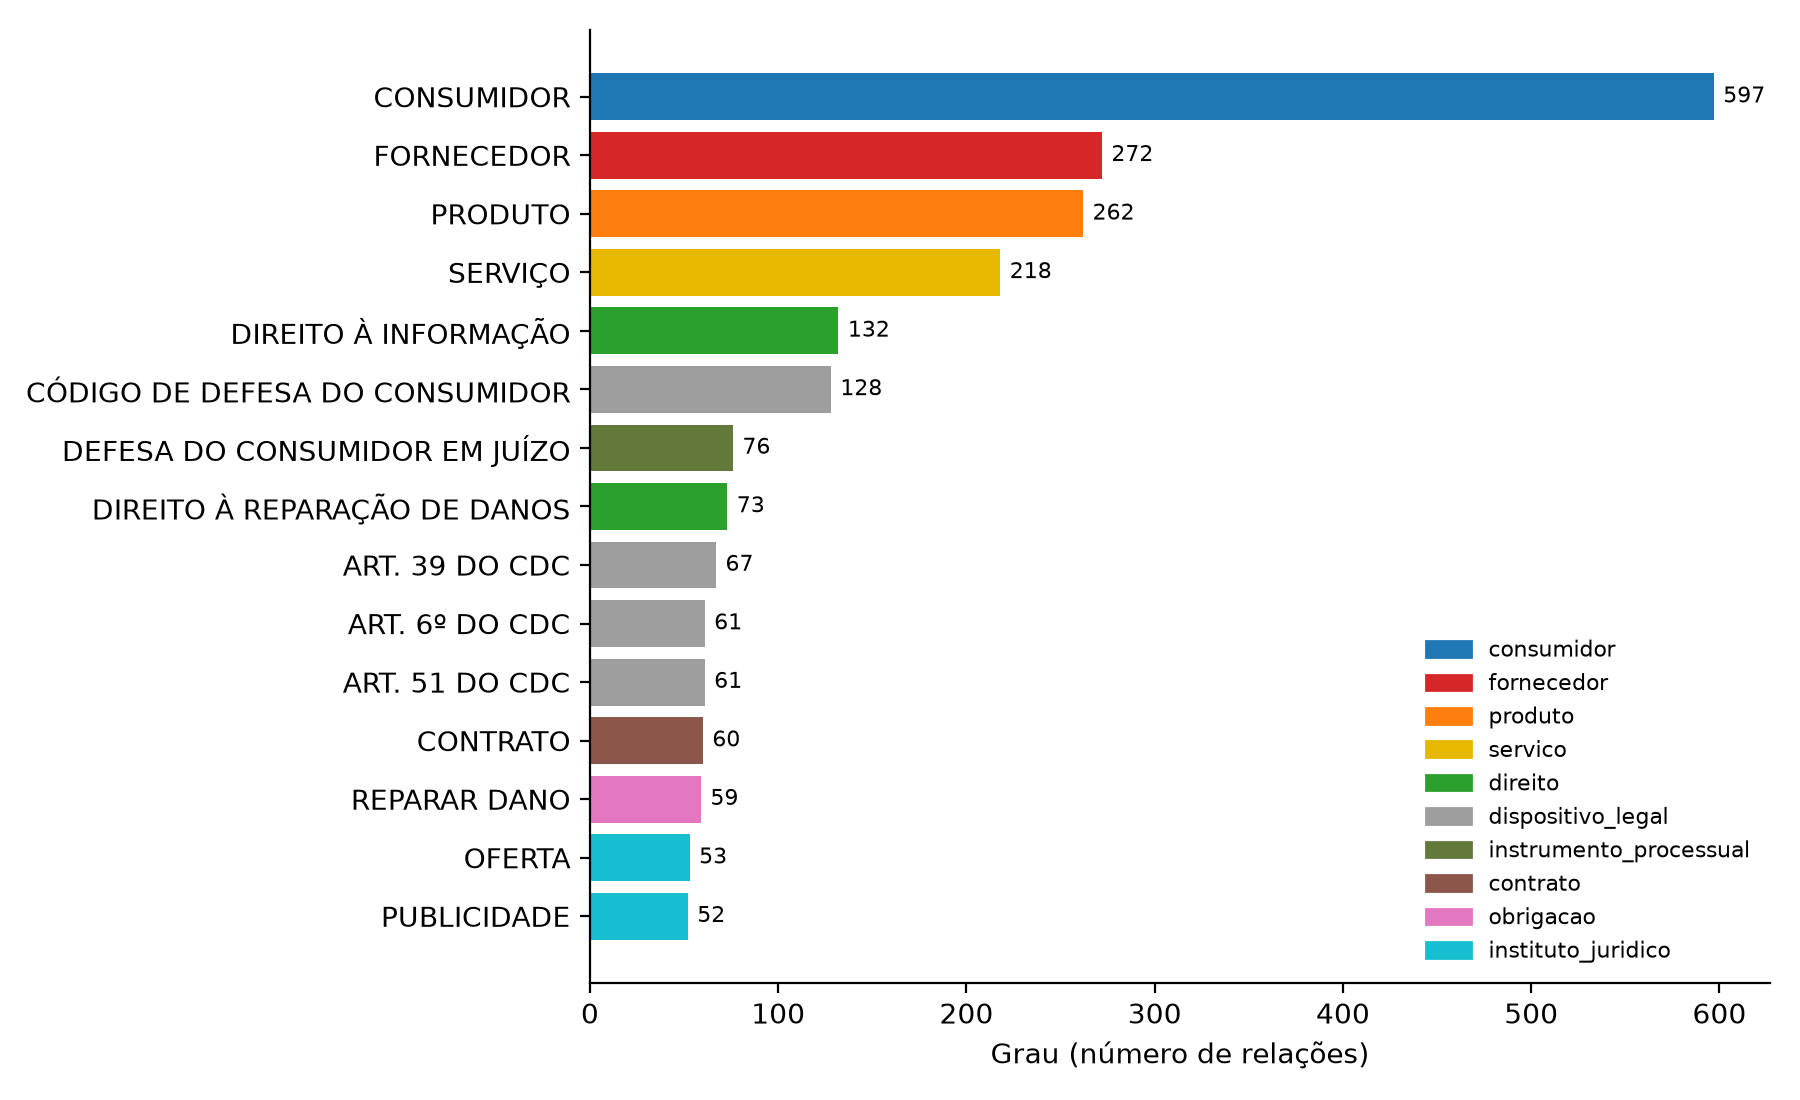
\includegraphics[width=.75\textwidth]{figuras/fig-grafo-graus.png}
\caption{As quinze entidades de maior grau do grafo do CDC, coloridas por tipo.}
\label{fig-grafo-graus}
\end{figure}

Essa concentração tem uma consequência para as buscas. Como as entidades centrais estão ligadas a quase tudo, elas aparecem no contexto de muitas consultas, mas acrescentam pouca informação específica; e, na busca local, as relações são ordenadas pelo grau combinado das entidades (Seção~\ref{sec-graphrag-indexacao-extracao}), o que favorece relações com as entidades centrais.

\subsection{Especialização em torno das entidades gerais}
\label{sec-analise-grafo-especializacao}

Filtrando o grafo na aplicação para exibir apenas os tipos consumidor, fornecedor, produto e serviço (Figura~\ref{fig-grafo-hubs}), observa-se uma estrutura que lembra a de uma hierarquia de classes: cada entidade geral é cercada por entidades menores que são casos particulares dela. A Figura~\ref{fig-grafo-especializacao} mostra essas estruturas em detalhe, considerando apenas as relações entre entidades do mesmo tipo.

\begin{figure}[htb]
\centering
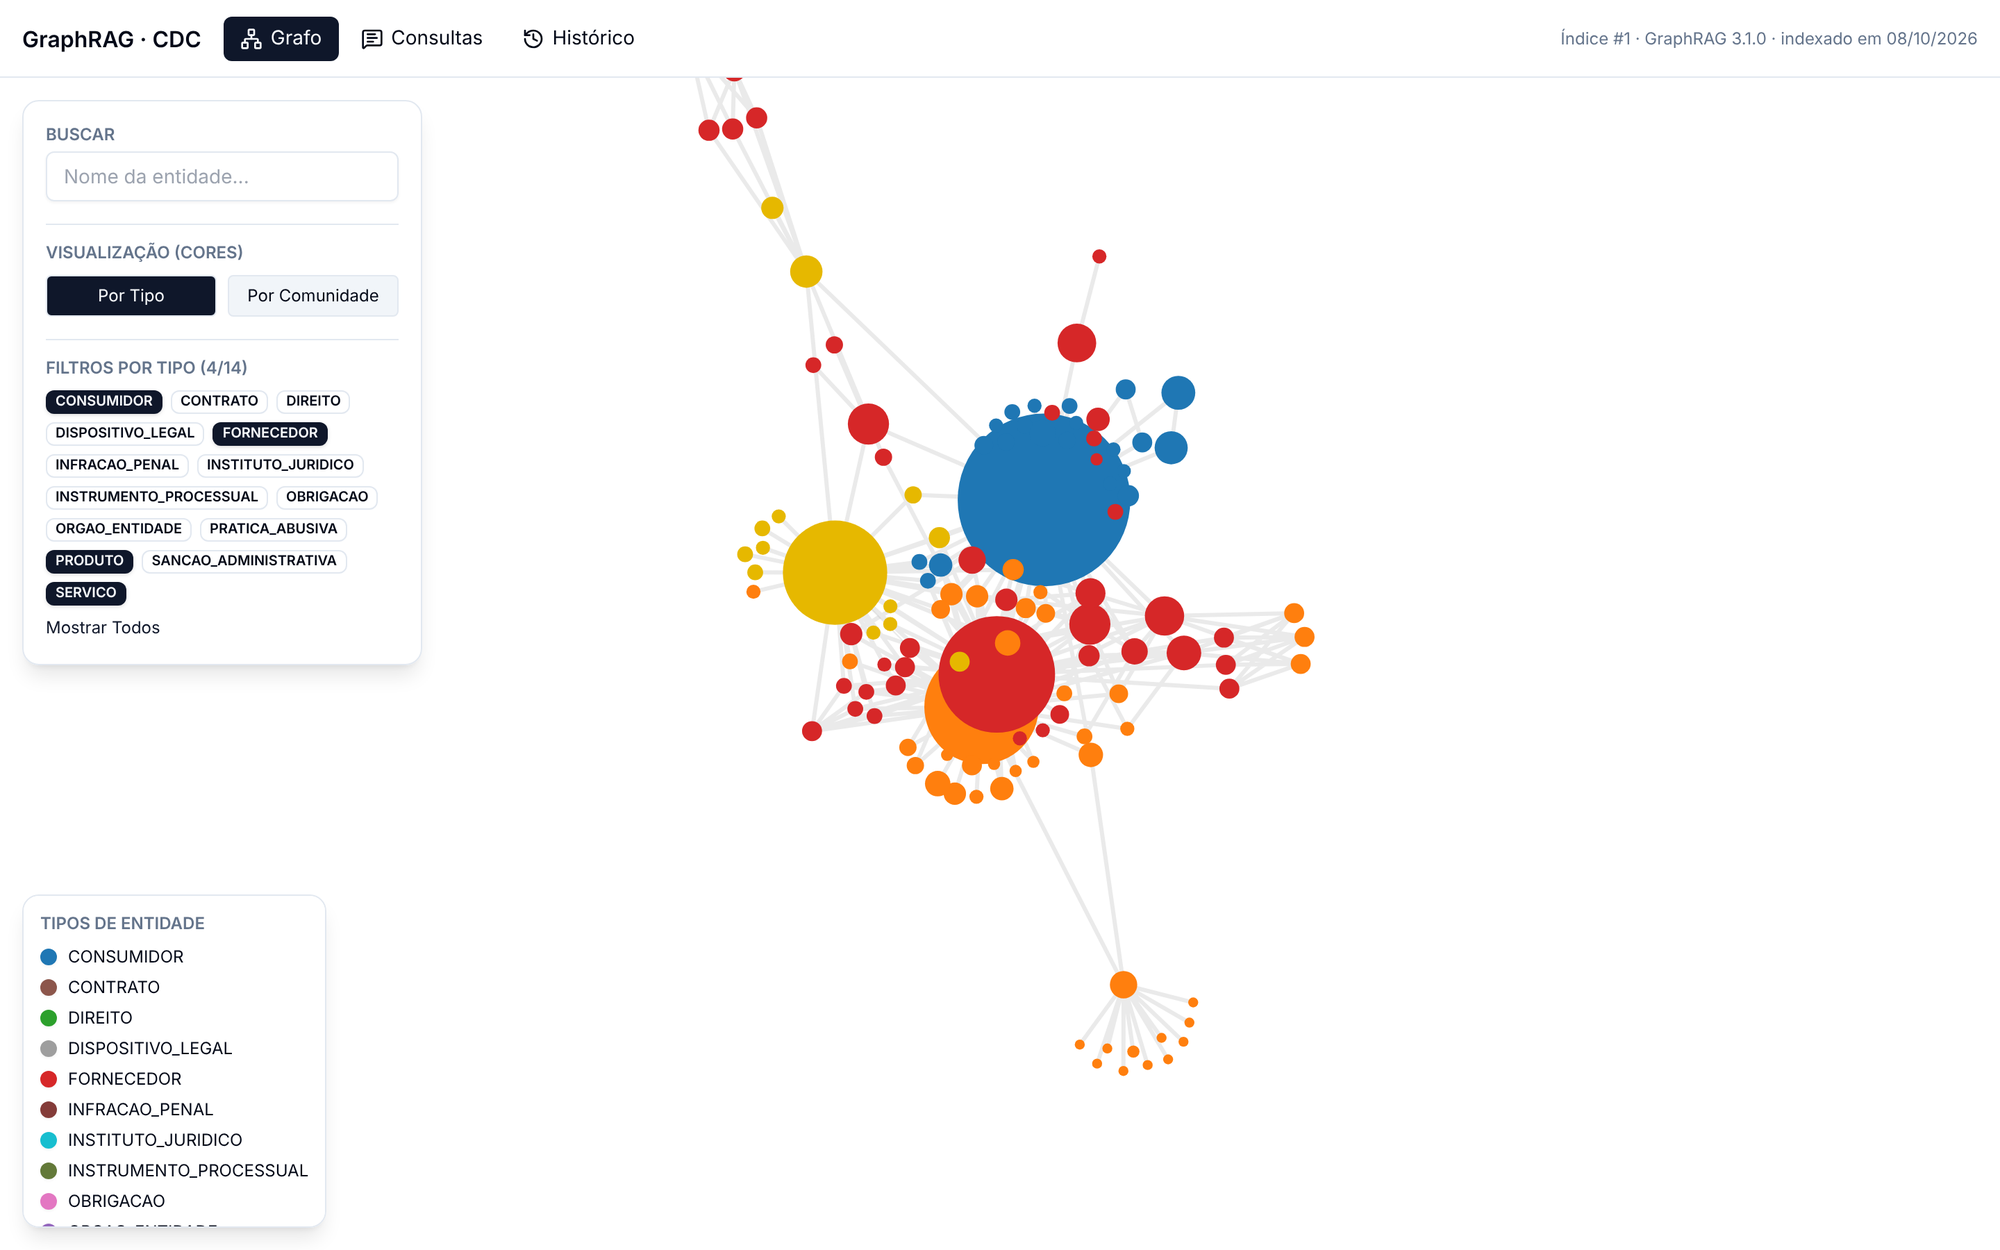
\includegraphics[width=.75\textwidth]{figuras/fig-grafo-hubs.png}
\caption{Aba Grafo filtrada para os tipos consumidor, fornecedor, produto e serviço: as quatro entidades gerais cercadas pelas entidades que as especializam.}
\label{fig-grafo-hubs}
\end{figure}

\begin{figure}[htbp]
\centering
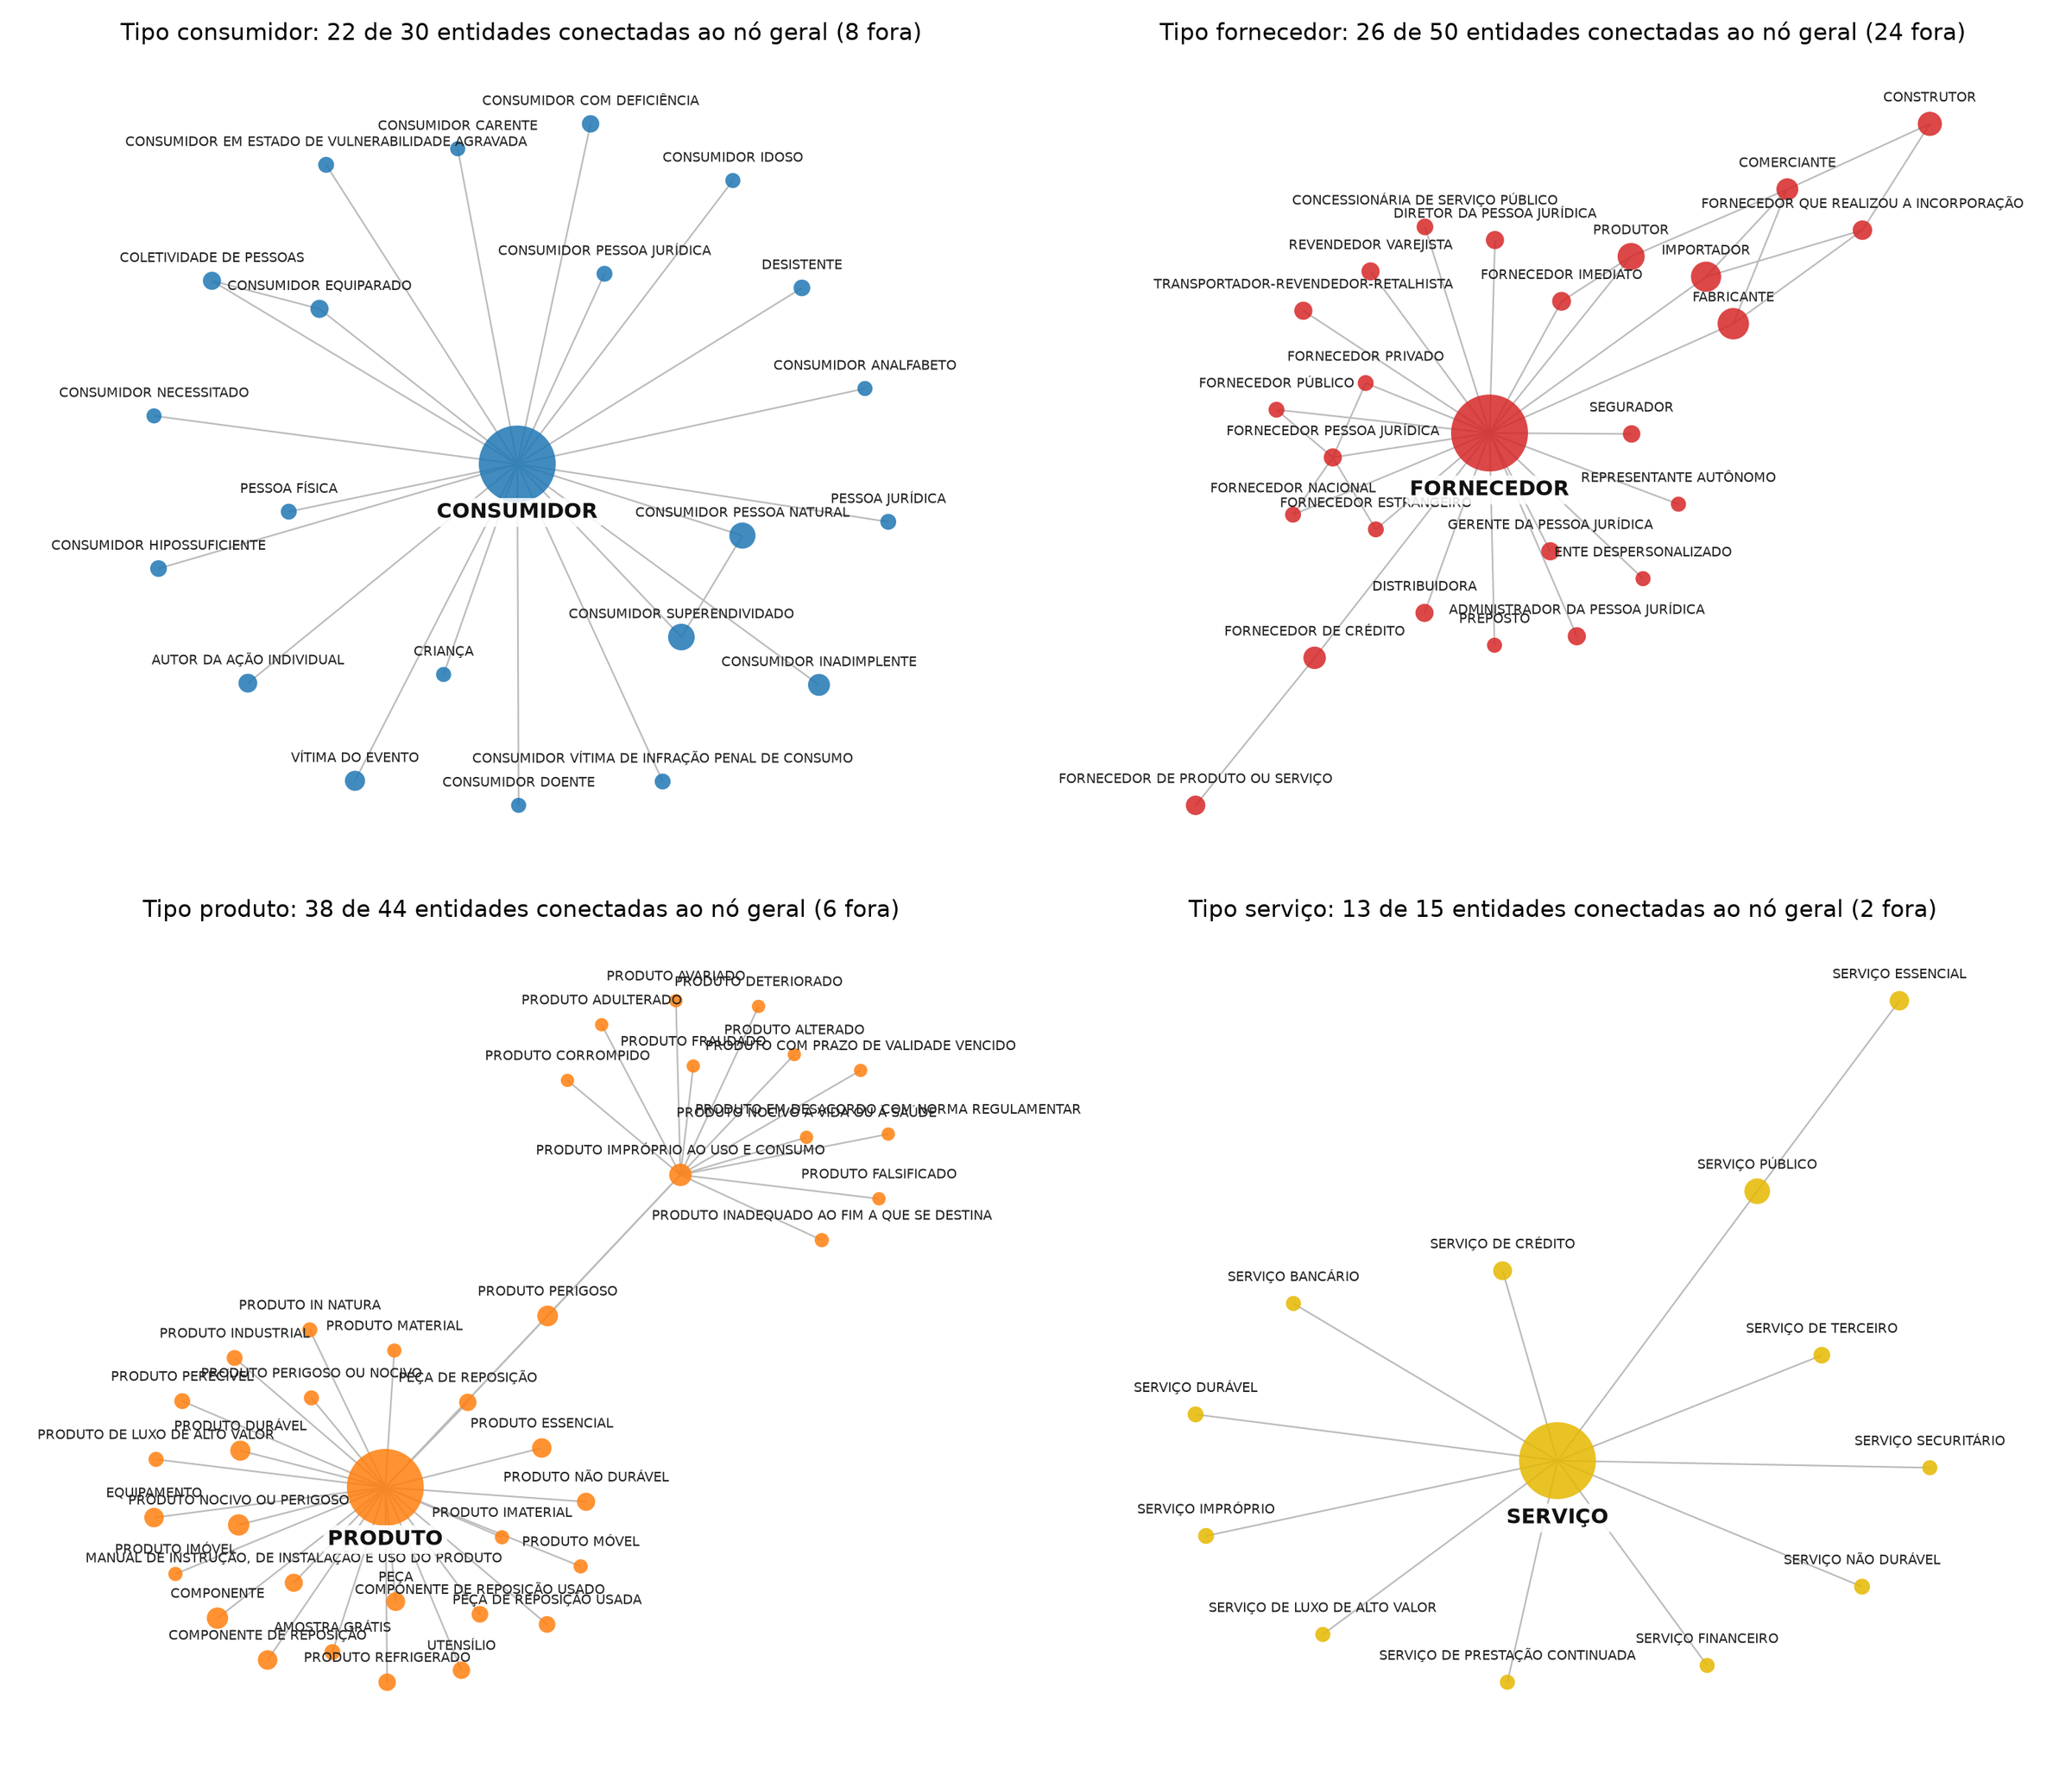
\includegraphics[width=.88\textwidth]{figuras/fig-grafo-especializacao.png}
\caption{Entidades de cada um dos tipos consumidor, fornecedor, produto e serviço e as relações entre elas. O tamanho dos nós é proporcional ao grau no grafo completo.}
\label{fig-grafo-especializacao}
\end{figure}

No tipo consumidor, a entidade geral CONSUMIDOR liga-se a especializações que correspondem a figuras previstas na lei -- CONSUMIDOR EQUIPARADO, COLETIVIDADE DE PESSOAS, VÍTIMA DO EVENTO, CONSUMIDOR SUPERENDIVIDADO -- e a situações de vulnerabilidade que o código protege de forma específica, como CONSUMIDOR IDOSO, CRIANÇA, CONSUMIDOR ANALFABETO e CONSUMIDOR COM DEFICIÊNCIA. No tipo fornecedor, FORNECEDOR liga-se às espécies enumeradas no art. 3º e nos artigos de responsabilidade -- FABRICANTE, PRODUTOR, CONSTRUTOR, IMPORTADOR, COMERCIANTE -- e a figuras introduzidas pelo tratamento do crédito, como FORNECEDOR DE CRÉDITO. O tipo produto apresenta dois níveis: PRODUTO é o centro de uma estrela (produto durável, não durável, perigoso, peça de reposição, amostra grátis), e PRODUTO IMPRÓPRIO AO USO E CONSUMO é o centro de outra, com as hipóteses do art. 18, § 6º (produto deteriorado, alterado, adulterado, avariado, falsificado, corrompido, fraudado, nocivo à vida ou à saúde, em desacordo com as normas regulamentares).

Essa estrutura não foi especificada em nenhum lugar: a taxonomia define apenas os tipos, e o \textit{prompt} de extração não pede relações de especialização. Ela emergiu da extração, porque o próprio texto da lei define os conceitos por gênero e espécie. Ao mesmo tempo, o grafo não distingue esse tipo de relação dos demais: a ligação entre CONSUMIDOR e CONSUMIDOR IDOSO é uma aresta como qualquer outra, com uma descrição em texto livre. Nem todas as especializações foram ligadas à entidade geral -- 8 das 30 entidades do tipo consumidor e 24 das 50 do tipo fornecedor não têm relação direta ou indireta com ela dentro do próprio tipo --, o que indica um limite da extração por trechos: a relação só é criada quando os dois conceitos aparecem no mesmo artigo.

\subsection{Relações, pesos e pontes entre artigos}
\label{sec-analise-grafo-relacoes}

As relações mais frequentes ligam dispositivos legais a institutos jurídicos (567 relações), a obrigações (280) e a direitos (257), o que reflete a forma como o grafo representa a lei: cada artigo é uma entidade ligada aos conceitos que ele trata. São também essas ligações que conectam artigos distantes no texto. A Figura~\ref{fig-grafo-ego} mostra a vizinhança da entidade DIREITO DE ARREPENDIMENTO: ela liga o art. 49, que cria o direito, ao art. 54-F, que, cinco capítulos adiante e incluído por outra lei, estende seus efeitos aos contratos de crédito conexos. No texto, nada aproxima os dois artigos além do assunto; no grafo, eles estão a dois passos de distância.

\begin{figure}[htb]
\centering
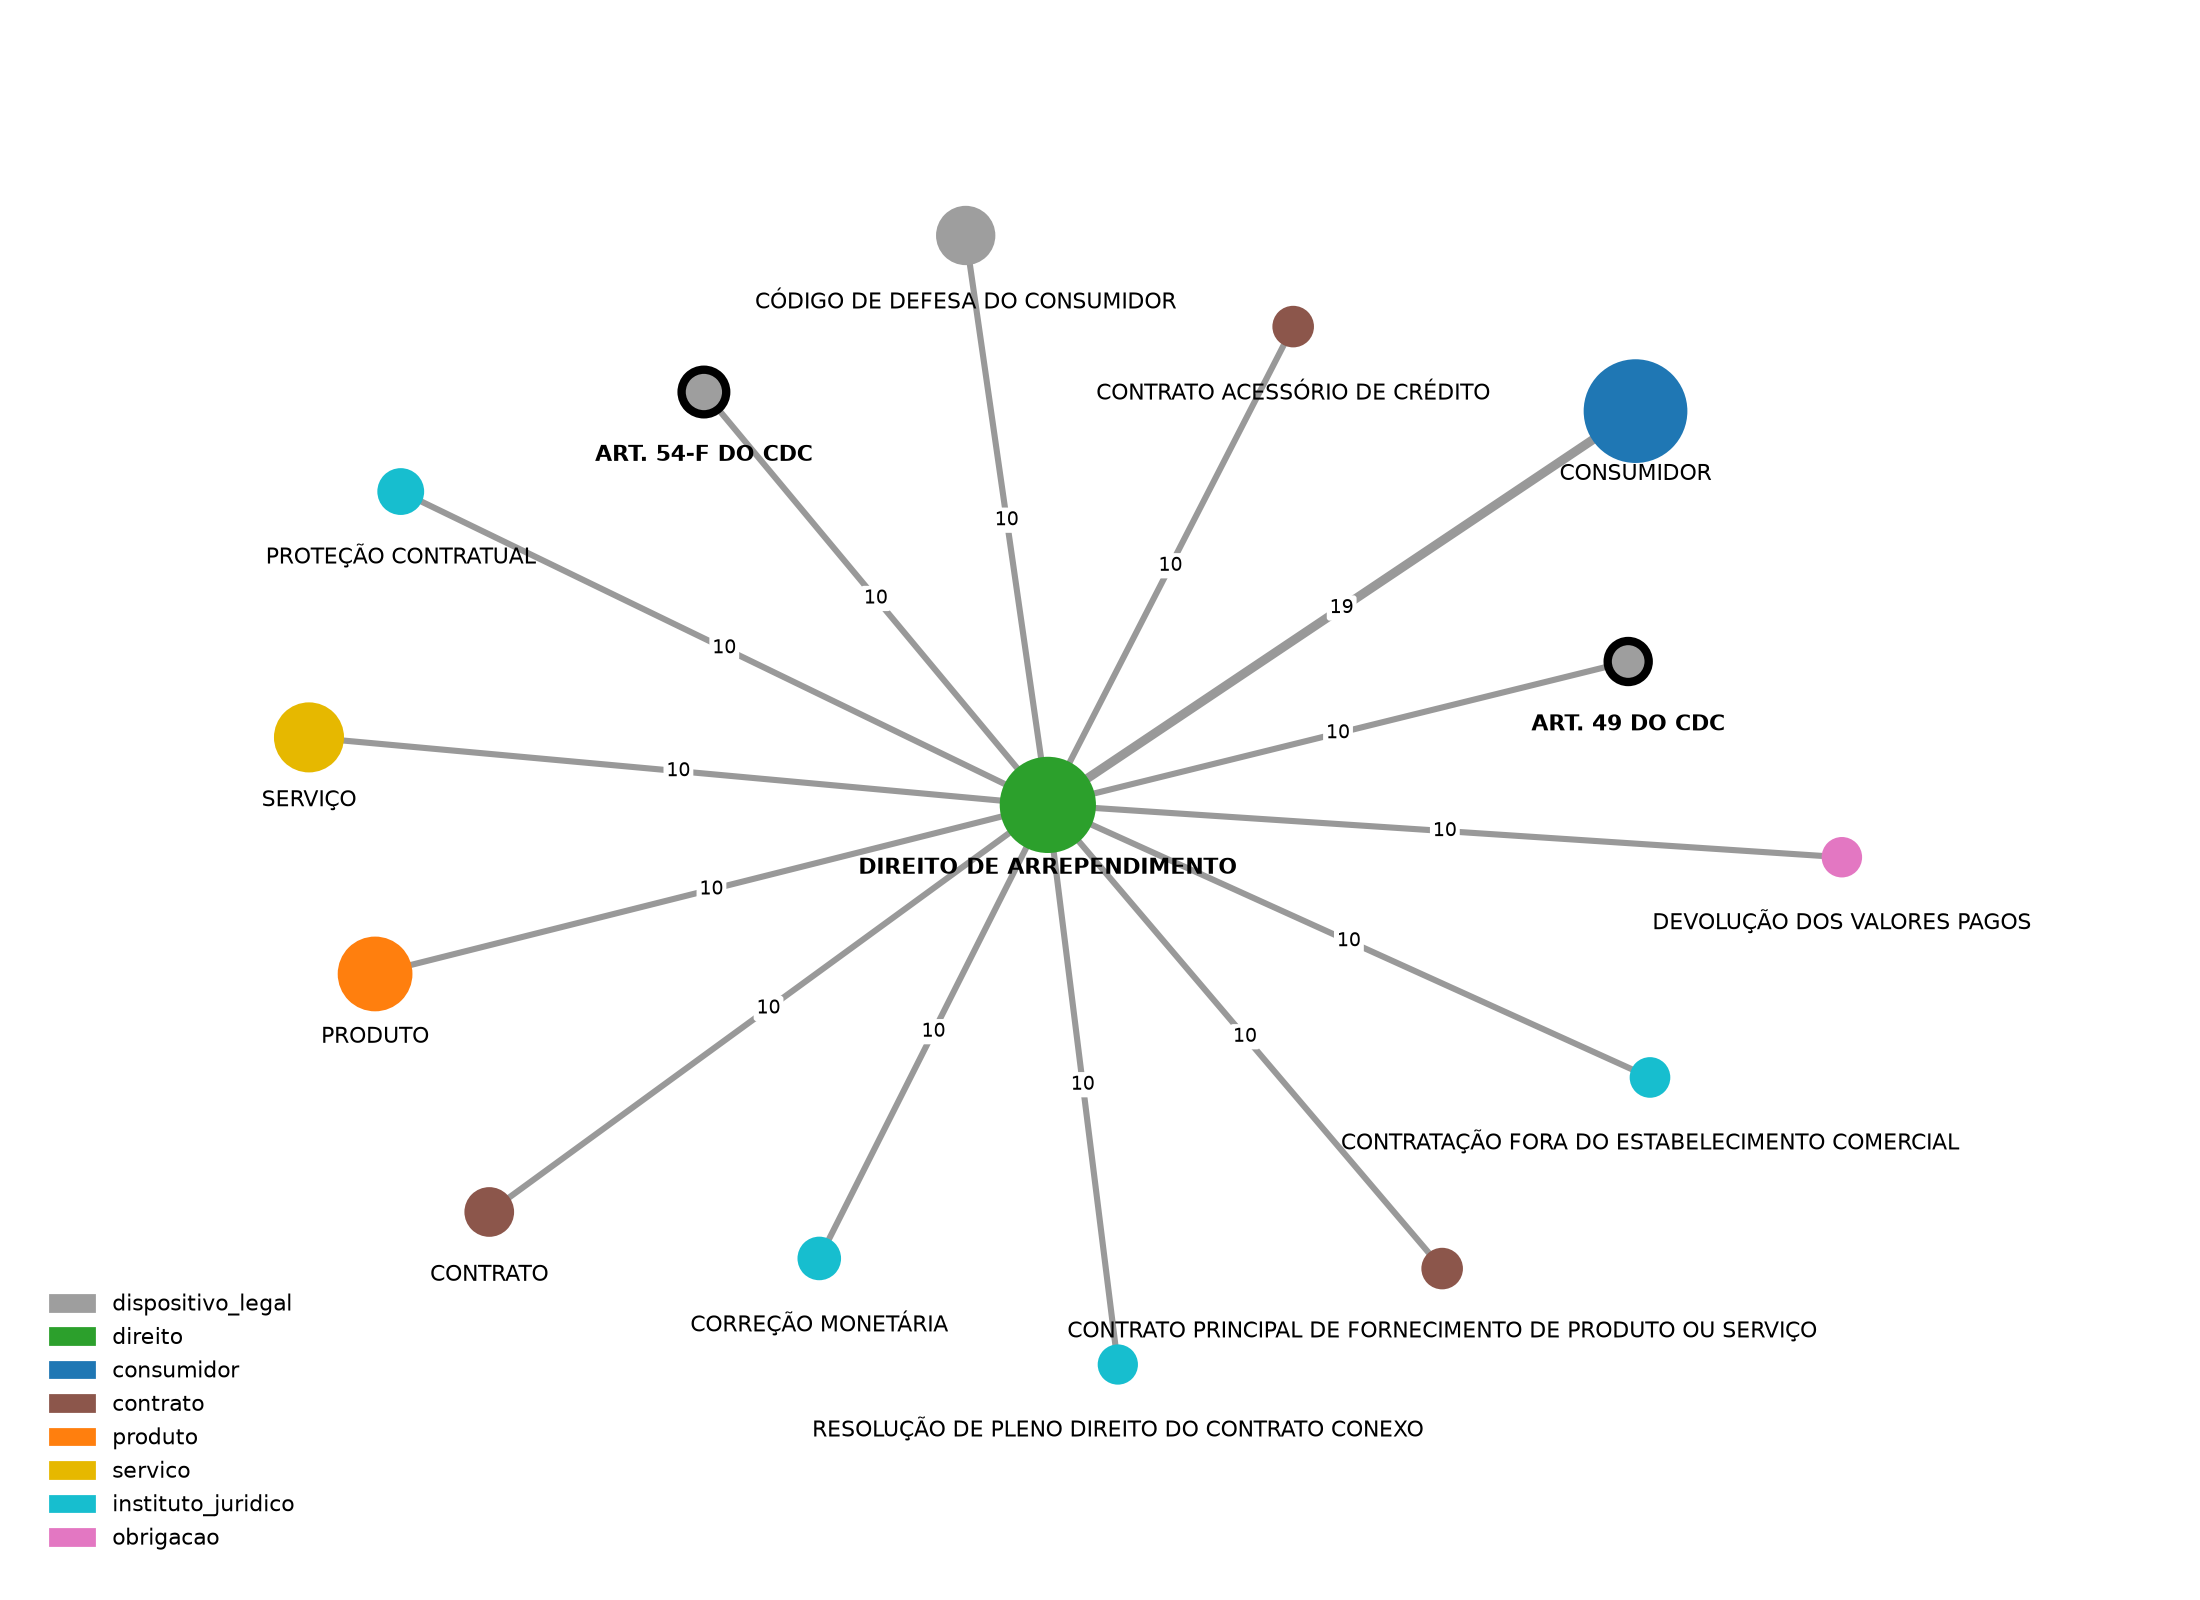
\includegraphics[width=.78\textwidth]{figuras/fig-grafo-ego-arrependimento.png}
\caption{Relações da entidade DIREITO DE ARREPENDIMENTO, com o peso de cada uma. Em destaque, os dois artigos que a mencionam.}
\label{fig-grafo-ego}
\end{figure}

A figura ilustra também como os pesos se comportam neste índice: quase todas as relações têm peso 10, a força máxima atribuída em uma única ocorrência, e a relação com CONSUMIDOR tem peso 19 porque aparece nos dois artigos. Como discutido na Seção~\ref{sec-graphrag-indexacao-extracao}, o peso funciona aqui, essencialmente, como uma contagem de ocorrências, e não como uma medida da intensidade da ligação.

Além dos artigos do CDC, o grafo representa as normas que o código menciona, e algumas delas funcionam como pontes entre partes distantes da lei: a LEI Nº 14.181/2021, que acrescentou o tratamento do superendividamento, liga os princípios e direitos básicos (arts. 4º a 6º) e os artigos sobre crédito do Título I (arts. 54-A a 54-G) aos artigos sobre a conciliação no superendividamento, no Título III (arts. 104-A a 104-C); e a LEI Nº 7.347/1985, da ação civil pública, liga as ações coletivas do Título III às disposições finais do Título VI, que alteram essa lei. Já a entidade CÓDIGO DE DEFESA DO CONSUMIDOR, com 128 relações com artigos e normas de todo o texto, funciona como um nó de ligação genérico, que pouco informa sobre o conteúdo.

\subsection{Comunidades}
\label{sec-analise-grafo-comunidades}

As comunidades do nível 0 (Tabela~\ref{tab-comunidades-n0} e Figura~\ref{fig-grafo-niveis}) correspondem a grandes temas do CDC -- tutela coletiva, superendividamento, sanções administrativas, tutela penal, vícios do produto, cadastros de consumidores --, mas não coincidem com a divisão formal da lei em títulos e capítulos. O direito de arrependimento, por exemplo, é criado no capítulo da proteção contratual, mas pertence, no nível 0, à comunidade do crédito ao consumidor, organizada em torno dos arts. 54-F e 54-G (Figura~\ref{fig-app-entidade}), o que reflete a ligação estabelecida pelo art. 54-F. O particionamento captura, portanto, uma organização temática transversal, que é a que interessa a quem pergunta sobre um assunto, e não sobre um capítulo. É essa organização que a busca global e o primer da DRIFT utilizam.

%%% Início de seção. %%%
\section{Roteiro de Análise das Consultas}
\label{sec-analise-roteiro}

Para cada consulta, a linha do tempo exibida pela aplicação (Seção~\ref{sec-aplicacao-frontend-consultas}) permite responder a um conjunto de perguntas sobre a recuperação:

\begin{enumerate}
    \item \textbf{O que foi recuperado?} As tabelas do contexto mostram, separadamente, as entidades, as relações, os relatórios de comunidade e os trechos de texto selecionados, com seus identificadores.
    \item \textbf{O que foi enviado ao modelo?} A etapa do \textit{prompt} mostra a mensagem de sistema final, com as instruções e o contexto já formatado, exatamente como o GraphRAG a monta, e o seu tamanho aproximado em \textit{tokens}.
    \item \textbf{Que parte do grafo esse contexto representa?} O subgrafo da consulta e o destaque no grafo completo mostram onde, no conhecimento extraído do CDC, o contexto se situa e quão concentrado ou disperso ele é.
    \item \textbf{O que a resposta usou do contexto?} As citações no formato \code{[Data: Sources (...)]} remetem aos identificadores das tabelas do contexto. Como cada unidade de texto corresponde a um artigo (Seção~\ref{sec-indexacao-segmentacao}), é possível saber quais artigos sustentam cada afirmação e quais artigos recuperados não foram usados.
    \item \textbf{Quanto custou?} As métricas mostram as chamadas ao modelo e os \textit{tokens} de entrada e saída, no total e por etapa.
\end{enumerate}

As seções a seguir aplicam esse roteiro a uma consulta de cada modalidade, na ordem crescente de complexidade.

%%% Início de seção. %%%
\section{Busca Básica: Recuperação por Similaridade}
\label{sec-analise-basic}

\textbf{Consulta:} ``O que acontece com o art. 54-E do CDC?'' -- 1 chamada, 4.452 \textit{tokens} de entrada, 123 de saída, 6,6 segundos.

\textbf{O que foi recuperado.} A busca básica recuperou as dez unidades de texto mais similares à pergunta (Figura~\ref{fig-app-contexto}, no Capítulo~\ref{sec-aplicacao}), correspondentes aos arts. 34, 53, 54, 54-B, 54-C, 54-D, 54-E, 54-F, 54-G e 85. O conjunto mostra como opera a similaridade vetorial: sete dos dez trechos pertencem ao capítulo do superendividamento, vizinhos do artigo pedido -- os metadados inseridos no início de cada trecho (Listagem~\ref{lst-chunk}), que repetem o nome do capítulo, contribuem para essa proximidade --, mas o art. 54-A, que abre o capítulo e define seus conceitos, não foi recuperado. O art. 85, de outro título, entrou por ser, como o 54-E, um artigo vetado cujo texto se resume à indicação do veto.

\textbf{O que foi enviado ao modelo.} Apenas texto: os dez trechos, com seus metadados, e as instruções. Um comportamento não documentado tornou-se visível aqui: a ordem dos trechos no \textit{prompt} é a ordem dos artigos no corpus, e não a ordem de similaridade. O código da busca básica converte os resultados da busca vetorial em um conjunto de identificadores e filtra a tabela de unidades de texto por esse conjunto, descartando o ranqueamento. Assim, o modelo não recebe nenhuma indicação de quais trechos são mais relevantes (defeito 12 da Tabela~\ref{tab-defeitos}).

\textbf{Que parte do grafo.} Embora a busca básica não use o grafo, o destaque mostra as entidades extraídas dos mesmos trechos: 160 entidades, espalhadas sobretudo pela região do grafo ligada ao crédito e ao superendividamento. Esse número contrasta com o que o modelo recebeu -- dez trechos de texto, sem nenhuma das relações que o grafo conhece entre eles.

\textbf{O que a resposta usou.} A resposta afirmou corretamente que o artigo foi vetado, que aparece no texto apenas como ``Art. 54-E. (VETADO)'' e que está associado à Lei nº 14.181/2021 e ao capítulo do superendividamento, citando apenas a unidade de texto do próprio artigo. O modelo ressalvou que os dados não informam a redação proposta nem os motivos do veto, comportamento desejável diante de um contexto que, de fato, não continha essa informação. Os outros nove trechos não foram utilizados. A resposta só foi possível porque o texto vetado foi mantido no corpus (Seção~\ref{sec-indexacao-corpus-vetados}).

%%% Início de seção. %%%
\section{Busca Local: Contexto a Partir das Entidades}
\label{sec-analise-local}

\textbf{Consulta:} ``O que diz o art. 49 do CDC sobre o direito de arrependimento?'' -- 1 chamada, 10.154 \textit{tokens} de entrada, 205 de saída, 8,6 segundos.

\textbf{O que foi recuperado.} O contexto da busca local é estruturado em tabelas:

\begin{itemize}
    \item \textbf{20 entidades}, selecionadas por similaridade entre a pergunta e as descrições: ``ART. 49 DO CDC'', ``DIREITO DE ARREPENDIMENTO'', ``DEVOLUÇÃO DOS VALORES PAGOS'', ``CONTRATAÇÃO FORA DO ESTABELECIMENTO COMERCIAL'', direitos relacionados ao desfazimento de contratos (reembolso da quantia paga, rescisão do contrato, desfazimento do negócio, cumprimento das declarações de vontade) e doze outros artigos (18, 19, 20, 24, 26, 35, 39, 46, 47, 48, 50 e 53);
    \item \textbf{9 relações}, todas partindo de ``ART. 49 DO CDC'': com CONSUMIDOR, PRODUTO, SERVIÇO, CONTRATO, PROTEÇÃO CONTRATUAL, CORREÇÃO MONETÁRIA, DIREITO DE ARREPENDIMENTO, CONTRATAÇÃO FORA DO ESTABELECIMENTO COMERCIAL e DEVOLUÇÃO DOS VALORES PAGOS;
    \item \textbf{17 trechos de texto}, os artigos de onde essas entidades foram extraídas: 49 em primeiro lugar, seguido do 54-F (contratos conexos, que também tratam do arrependimento), dos artigos vizinhos da proteção contratual (46, 47, 48, 50, 51, 53 e 54) e de artigos sobre vícios, oferta e práticas abusivas (18, 19, 20, 24, 26, 35, 39 e 41);
    \item \textbf{nenhum relatório de comunidade}.
\end{itemize}

A ausência de relatórios foi outro achado que a ferramenta tornou visível. Com os valores padrão, a busca local reserva 15\% do contexto (1.800 \textit{tokens}) para os relatórios de comunidade, e todos os relatórios deste índice são maiores que isso: o menor tem cerca de 1.300 \textit{tokens}, e a mediana, cerca de 2.300. Como a montagem do contexto não trunca relatórios, nenhum é incluído (defeito 13 da Tabela~\ref{tab-defeitos}). Ou seja, com a configuração padrão e relatórios do tamanho gerado neste trabalho, a busca local usa entidades, relações e trechos, mas não a visão de comunidade.

\textbf{O que foi enviado ao modelo.} Cerca de nove mil \textit{tokens} de contexto e instruções (Figura~\ref{fig-analise-prompt}), mais que o dobro da busca básica, organizados em tabelas com identificadores que o modelo deve citar.

\begin{figure}[htbp]
\centering
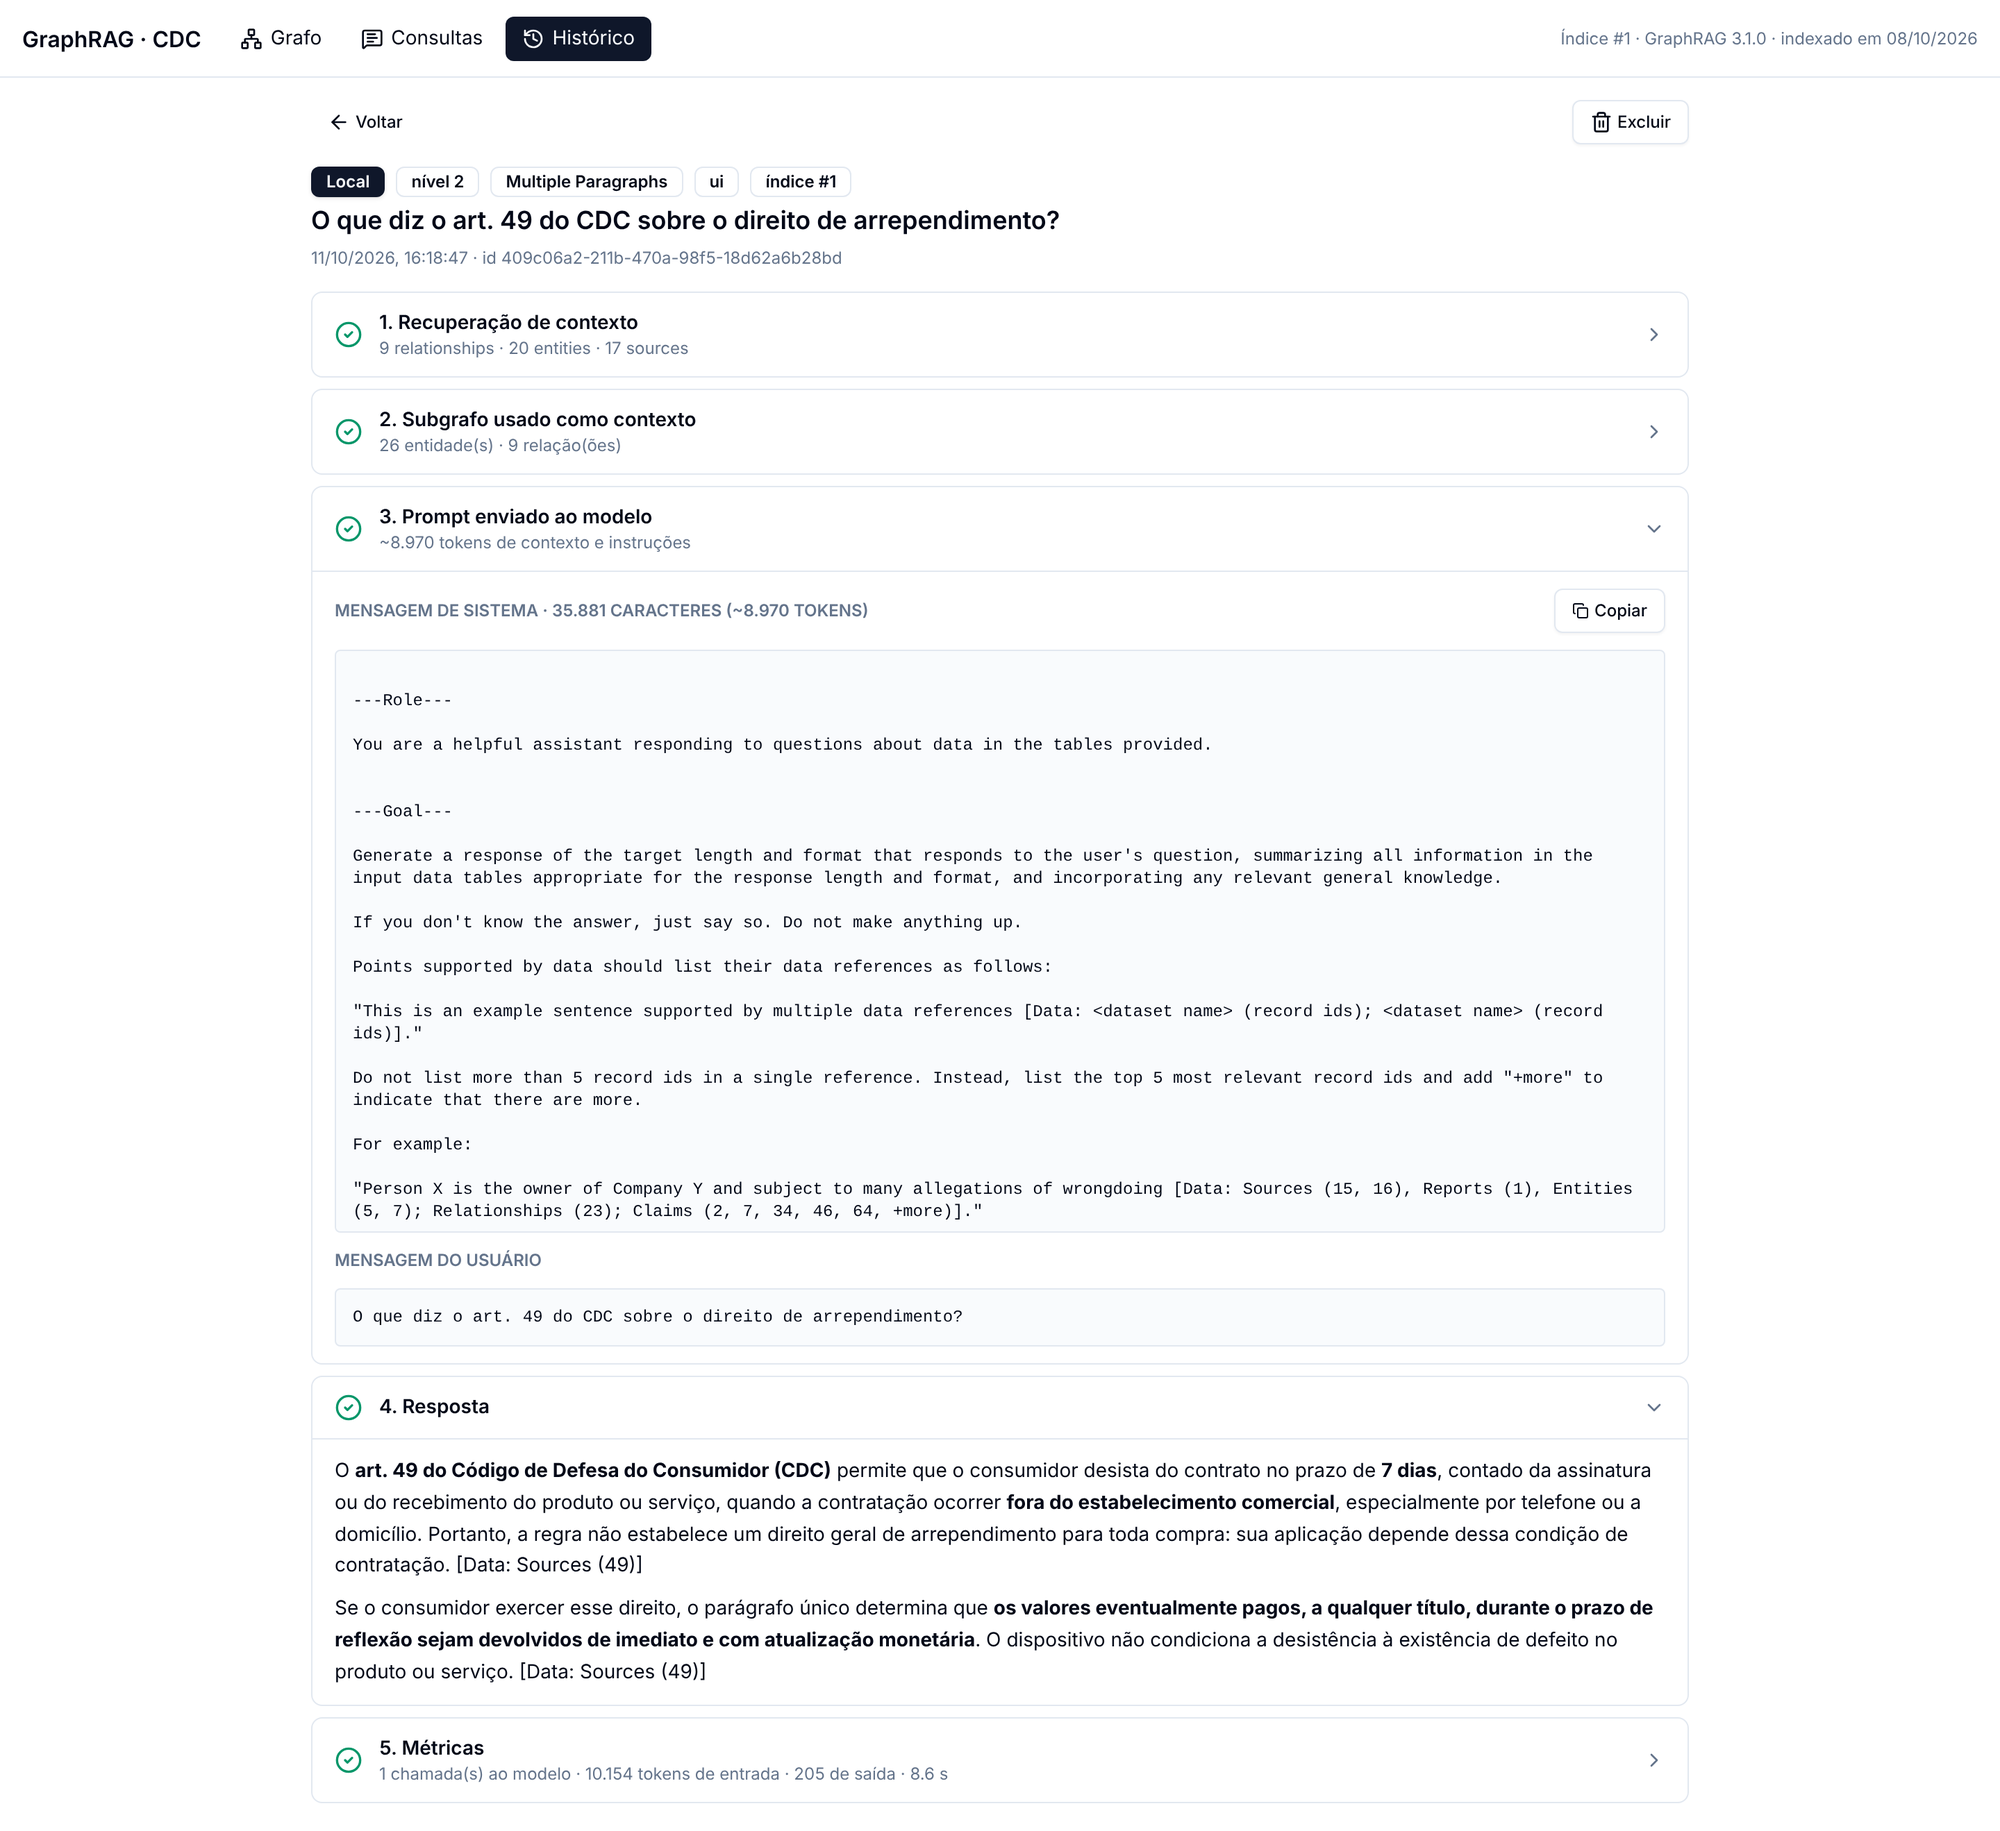
\includegraphics[width=.7\textwidth]{figuras/fig-app-local-prompt.png}
\caption{Etapa do \textit{prompt} enviado ao modelo na consulta da busca local sobre o art. 49: instruções seguidas das tabelas de entidades, relações e trechos.}
\label{fig-analise-prompt}
\end{figure}

\textbf{Que parte do grafo.} O destaque (Figura~\ref{fig-app-destaque}, no Capítulo~\ref{sec-aplicacao}) mostra um contexto concentrado: 26 entidades -- as 20 da tabela e 6 que só aparecem como extremidade das relações, como CONSUMIDOR e PRODUTO -- e 9 relações, formando uma estrela em torno do art. 49, cercada pelos artigos vizinhos da proteção contratual e pelos artigos sobre vícios. É a vizinhança do artigo no grafo, e não apenas os trechos de vocabulário parecido.

\textbf{O que a resposta usou.} A resposta descreveu corretamente o prazo de sete dias, a condição de contratação fora do estabelecimento comercial e a devolução imediata e atualizada dos valores pagos, ressaltando que a regra não cria um direito geral de arrependimento para toda compra, e citou apenas a unidade de texto do art. 49. O contexto oferecia conexões que a resposta não explorou, como a extensão do arrependimento aos contratos conexos prevista no art. 54-F. Para uma pergunta pontual sobre o conteúdo de um artigo, isso é adequado. Mas o exemplo mostra que um contexto mais rico não se traduz automaticamente em uma resposta mais rica: o que o modelo usa depende também da pergunta e das instruções do \textit{prompt}.

%%% Início de seção. %%%
\section{Busca DRIFT: Exploração Iterativa}
\label{sec-analise-drift}

\textbf{Consulta:} ``Quais são os direitos básicos do consumidor?'' -- configuração padrão, nível de comunidade 2; 67 chamadas, 524.646 \textit{tokens} de entrada, 62.925 de saída, 221 segundos.

\textbf{O que foi recuperado.} A DRIFT é a modalidade em que a inspeção das etapas mais revela, porque ela própria decide o que pesquisar. As etapas registradas mostram:

\begin{itemize}
    \item \textbf{Primer}: os 20 relatórios de comunidade mais similares à resposta hipotética foram divididos em cinco grupos; cada grupo produziu uma resposta parcial -- todas centradas no art. 6º -- e uma lista de perguntas de acompanhamento. Foram geradas 28 perguntas, como ``Quais informações o fornecedor deve apresentar sobre produtos e serviços?'', ``Quando uma cláusula contratual é considerada abusiva pelo CDC?'' e ``Quais são os prazos para reclamar de vícios em produtos?''.
    \item \textbf{Aprofundamento}: em três rodadas, 60 perguntas foram respondidas, cada uma por uma busca local completa, e cada resposta gerou novas perguntas. A Tabela~\ref{tab-drift-arvore} mostra a árvore resultante: 502 perguntas, das quais 61 respondidas (incluindo a original). As perguntas se afastam da original à medida que a árvore se aprofunda: no terceiro nível aparecem perguntas como ``Quais são as penas pela omissão de advertências sobre riscos?'' e ``Como registrar uma reclamação no Procon ou ingressar no Juizado Especial Cível?''.
    \item \textbf{Contexto das buscas locais}: nas 60 buscas locais, o contexto continha \textbf{apenas trechos de texto} -- nenhuma entidade, relação ou relatório (defeito 7 da Tabela~\ref{tab-defeitos}). Somadas, as buscas recuperaram 1.189 trechos, com muitas repetições, cobrindo 116 dos 130 artigos do CDC; os mais frequentes foram os arts. 18 (36 vezes), 35, 20, 6º, 19 e 51.
    \item \textbf{Redução}: as 61 respostas parciais, cerca de 49 mil \textit{tokens}, foram enviadas a uma chamada final.
\end{itemize}

\begin{table}[htb]
\centering
\caption{Árvore de perguntas da consulta DRIFT, por profundidade.}
\label{tab-drift-arvore}
\footnotesize
\begin{tabular}{L{6cm} r r r}
\toprule
\textbf{Profundidade} & \textbf{Perguntas geradas} & \textbf{Respondidas} & \textbf{Não respondidas} \\
\midrule
0 (pergunta original) & 1 & 1 & 0 \\
1 (geradas pelo primer) & 28 & 21 & 7 \\
2 & 176 & 30 & 146 \\
3 & 234 & 9 & 225 \\
4 & 63 & 0 & 63 \\
\midrule
\textbf{Total} & \textbf{502} & \textbf{61} & \textbf{441} \\
\bottomrule
\end{tabular}
\end{table}

\textbf{Que parte do grafo.} Com a configuração padrão, a DRIFT usa o grafo apenas no primer, por meio dos relatórios de comunidade; o aprofundamento é, na prática, uma sequência de buscas por trechos de texto guiada por perguntas geradas pelo modelo. Por isso, o subgrafo exibido pela aplicação para essa consulta é vazio. Esse resultado não seria perceptível pela resposta, que é extensa e correta, nem pelas métricas: só a inspeção do contexto de cada busca local o revelou.

\textbf{O que a resposta usou.} A resposta final organizou os direitos básicos do art. 6º em grupos temáticos (segurança, educação e informação; proteção contra abusos e equilíbrio contratual; reparação de danos e acesso à defesa; serviços públicos e proteção financeira) e acrescentou outros direitos relevantes na prática, como a garantia legal e o direito de arrependimento. As citações remetem ao art. 6º e, no último bloco, aos arts. 18, 20, 24, 30 e 49. Ou seja, das dezenas de artigos explorados, poucos chegaram à resposta, o que é esperado em uma síntese, mas indica que boa parte do custo da exploração não se refletiu no resultado.

\textbf{Quanto custou.} A etapa de aprofundamento respondeu por 417 mil dos 525 mil \textit{tokens} de entrada (cerca de sete mil por busca local), o primer por 56 mil e a redução por 49 mil. A consulta custou, em \textit{tokens} de entrada, cerca de cinquenta vezes a busca local. A análise das opções de configuração da DRIFT (Seção~\ref{sec-graphrag-config-consultas}) mostra que é possível reduzir esse custo diminuindo o número de perguntas por rodada e de rodadas, e fazer as buscas locais usarem o grafo ajustando as proporções de contexto.

%%% Início de seção. %%%
\section{Busca Global: Síntese a Partir das Comunidades}
\label{sec-analise-global}

Na busca global, a ferramenta exibe as etapas do \textit{map-reduce}: os relatórios de comunidade considerados, os lotes enviados ao modelo, os pontos-chave de cada lote ordenados pela nota de importância e com o lote de origem, o \textit{prompt} da síntese e a resposta final. O destaque no grafo mostra as comunidades cujos relatórios foram efetivamente citados nos pontos-chave relevantes e na resposta, o que permite distinguir as comunidades lidas das comunidades usadas.

Nesta versão do trabalho, a busca global foi exercitada com o índice real e com os modelos simulados da biblioteca, o que permitiu medir o tamanho do contexto em cada nível da hierarquia sem custo de geração (Tabela~\ref{tab-global-niveis}). Os números mostram que, para a busca global, o nível de comunidade é a principal decisão de análise: no nível 0, o modelo lê 17 relatórios amplos, que correspondem aos grandes temas do CDC (Tabela~\ref{tab-comunidades-n0}); nos níveis mais profundos, lê centenas de relatórios específicos, com custo mais de dez vezes maior. A análise qualitativa de consultas globais reais, nos diferentes níveis, fica como trabalho futuro.

\begin{table}[htb]
\centering
\caption{Tamanho do contexto da busca global por nível de comunidade, medido no índice do CDC.}
\label{tab-global-niveis}
\footnotesize
\begin{tabular}{L{4cm} r r}
\toprule
\textbf{Nível de comunidade} & \textbf{Chamadas ao modelo} & \textbf{\textit{Tokens} de entrada} \\
\midrule
0 & 7 & 71 mil \\
1 & 30 & 336 mil \\
2 (padrão) & 68 & 775 mil \\
3 & 82 & 944 mil \\
\bottomrule
\end{tabular}
\end{table}

%%% Início de seção. %%%
\section{Síntese}
\label{sec-analise-sintese}

A Tabela~\ref{tab-analise-sintese} resume o que a ferramenta mostrou sobre o contexto de cada modalidade nas consultas analisadas.

\begin{table}[htb]
\centering
\caption{Síntese do contexto enviado ao modelo em cada modalidade, nas consultas analisadas.}
\label{tab-analise-sintese}
\footnotesize
\begin{tabular}{L{1.5cm} L{4.4cm} L{3.2cm} L{4.8cm}}
\toprule
\textbf{Busca} & \textbf{Contexto enviado ao modelo} & \textbf{Chamadas / \textit{tokens} de entrada} & \textbf{O que a inspeção revelou} \\
\midrule
Básica & 10 trechos, sem estrutura & 1 / 4,5 mil & Trechos vizinhos ao artigo pedido; ordem de similaridade descartada; artigo central do capítulo não recuperado \\
Local & 20 entidades, 9 relações e 17 trechos em tabelas & 1 / 10 mil & Vizinhança do artigo no grafo; nenhum relatório de comunidade por falta de espaço; resposta usou só o artigo central \\
DRIFT & Relatórios (primer); 60 contextos só com trechos; 61 respostas parciais (redução) & 67 / 525 mil & Grafo usado só no primer; cobertura de 116 artigos; perguntas cada vez mais distantes da original; custo concentrado no aprofundamento \\
Global & Lotes de relatórios de comunidade & 7 a 82 / 71 a 944 mil (por nível) & Custo determinado pelo nível de comunidade \\
\bottomrule
\end{tabular}
\end{table}

Três observações gerais emergem desses exemplos. A primeira é que as modalidades diferem muito mais no que enviam ao modelo do que se percebe pelas respostas: as três respostas analisadas são corretas, mas se apoiam em contextos de natureza, tamanho e custo muito diferentes. A segunda é que a configuração padrão do GraphRAG, combinada às características do índice -- em particular, relatórios de comunidade maiores que o espaço reservado a eles --, faz com que partes da estrutura de grafo simplesmente não cheguem ao modelo na busca local e na DRIFT, sem nenhum aviso. A terceira é que esses comportamentos só puderam ser identificados porque a aplicação expõe, para cada consulta, o contexto e o \textit{prompt} efetivamente utilizados. Essa é a principal contribuição da prova de conceito como ferramenta: tornar a recuperação observável, o que é condição para qualquer comparação criteriosa entre as modalidades.
